\documentclass{beamer}
\usepackage{style}

\title{M05 - Mini project}
\subtitle{Human Activity Recognition from Continuous Ambient Sensor Data}
\author{Steve Devènes, Amara Spano}
\institute{Unidistance}
\date{\today}
\usetheme{Madrid}

\begin{document}

	\begin{frame}
		\titlepage
	\end{frame}

	% \begin{frame}
	% 	\frametitle{Outline}
	% 	\tableofcontents
	% \end{frame}

%	\begin{frame}
%		\frametitle{Selected project}
%	\end{frame}

	\begin{frame}
		\frametitle{Working hypothesis}
		It's possible to perform human activity recognition from continuous ambient sensor data.
	\end{frame}

	\begin{frame}
		\frametitle{Data}
		\begin{itemize}
			\item Data is available online on the UC Irvine machine learning repository(Dua, D. and Graff, C. (2019). UCI Machine Learning Repository [http://archive.ics.uci.edu/ml]. Irvine, CA: University of California, School of Information and Computer Science.).
			\item Data are downloaded through the command line.
			\item The dataset is large, it contains 36 features measured plus one output for the classification label
			of the activity (35 different activities), for a total of 13956534 entries (30 different participants).
			\item For the experiments, data from a unique house is used
			\item There are two evaluation protocols splitting the data into 80\% train and 20\% test sets with 2 different random seeds.
		\end{itemize}
	\end{frame}

	\begin{frame}
		\frametitle{Workflow}
		For different experiments:
		\begin{enumerate}
			\item Load the training data
			\item Create and train a random forest classifier
			\item Load the test data
			\item Make prediction on test data
			\item Print the confusion matrix for the model evaluation. Confusion matrices are also available in graphs with plotly.express.
		\end{enumerate}

		The experiments run sequentially.
	\end{frame}

	\begin{frame}
		\frametitle{Version control}
		On github at \url{https://github.com/sdevenes/M05_MiniProject}

		The work is organized using github issues to create and assign tasks.

		The general approach:
		\begin{itemize}
			\item Create 1 branch per feature named \textit{feature/feature\_name} or \textit{issue\_\#issue/issue\_name} 
			\item When the feature is complete, do a pull request with the other as a reviewer
		\end{itemize}

		\begin{figure}
			\centering
			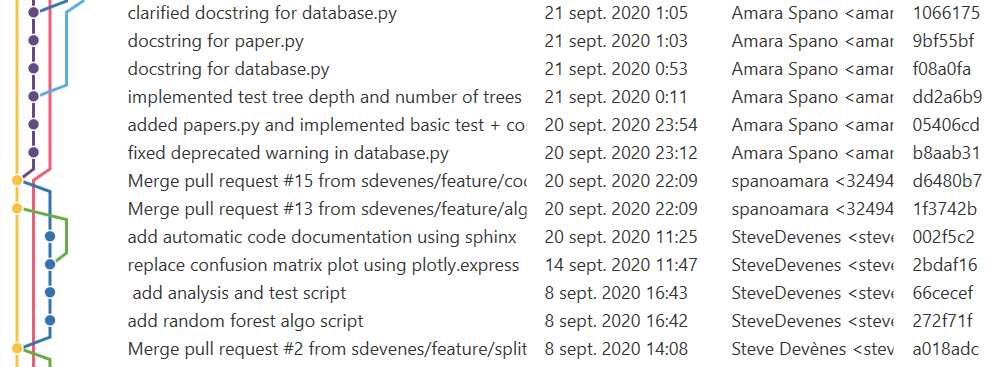
\includegraphics[width=\linewidth]{img/git_tree.png}
		\end{figure}
	\end{frame}


	\begin{frame}
		\frametitle{Unit Testing and CI}
		\begin{itemize}
			
			\item The majority of the functions in the code are covered by unit-tests for a total coverage of 86\%,
			this was done using Nose python package.
			\url{https://coveralls.io/github/sdevenes/M05_MiniProject?branch=master}
			\item These tests are ran at each commit through travis CI:
			\url{https://travis-ci.org/github/sdevenes/M05_MiniProject}
			Procuring a quick detection of bugs and e\_ors that could appears
			during the project development.
			\item Black is used to enforce formatting that conforms to PEP 8. The formatting is also tested with travis CI.
		\end{itemize}
	\end{frame}

	\begin{frame}
		\frametitle{Documentation}
		Each function is commented with a docstring. The documentation is
		then build automatically in the CI using Sphinx at each new commit on the
		master branch.

		Doc available here: \url{https://sdevenes.github.io/M05_MiniProject/index.html}
	\end{frame}

	\begin{frame}
		\frametitle{Packaging and Deployment}
		\begin{itemize}
			\item 
			The package is deployed under \textit{rr\_sdas} version 0.2.0 on pypitest.
			\url{https://test.pypi.org/project/rr-sdas/0.2.0/}
			\item The package is composed of 3 sub-packages:
				\begin{enumerate}
					\item download\_data
					\item experiment
					\item tests
				\end{enumerate}
			\item The experiments are configurable through:
				\begin{enumerate}
					\item Command line arguments (file sources and destination)
					\item \textit{experiment.ini} for the random forest parameters
				\end{enumerate}
			\item The project is licensed under an MIT license as it is an open source license and it is less restrictive than a GPL license.
		\end{itemize}
		
	\end{frame}

\end{document}
